\documentclass{extbook}[14pt]
\usepackage{multicol, enumerate, enumitem, hyperref, color, soul, setspace, parskip, fancyhdr, amssymb, amsthm, amsmath, latexsym, units, mathtools}
\everymath{\displaystyle}
\usepackage[headsep=0.5cm,headheight=0cm, left=1 in,right= 1 in,top= 1 in,bottom= 1 in]{geometry}
\usepackage{dashrule}  % Package to use the command below to create lines between items
\newcommand{\litem}[1]{\item #1

\rule{\textwidth}{0.4pt}}
\pagestyle{fancy}
\lhead{}
\chead{Answer Key for Makeup Progress Quiz 2 Version C}
\rhead{}
\lfoot{5763-3522}
\cfoot{}
\rfoot{Spring 2021}
\begin{document}
\textbf{This key should allow you to understand why you choose the option you did (beyond just getting a question right or wrong). \href{https://xronos.clas.ufl.edu/mac1105spring2020/courseDescriptionAndMisc/Exams/LearningFromResults}{More instructions on how to use this key can be found here}.}

\textbf{If you have a suggestion to make the keys better, \href{https://forms.gle/CZkbZmPbC9XALEE88}{please fill out the short survey here}.}

\textit{Note: This key is auto-generated and may contain issues and/or errors. The keys are reviewed after each exam to ensure grading is done accurately. If there are issues (like duplicate options), they are noted in the offline gradebook. The keys are a work-in-progress to give students as many resources to improve as possible.}

\rule{\textwidth}{0.4pt}

\begin{enumerate}\litem{
Construct the lowest-degree polynomial given the zeros below. Then, choose the intervals that contain the coefficients of the polynomial in the form $ax^3+bx^2+cx+d$.
\[ \frac{-2}{5}, 3, \text{ and } \frac{7}{4} \]The solution is \( 20x^{3} -87 x^{2} +67 x + 42 \), which is option B.\begin{enumerate}[label=\Alph*.]
\item \( a \in [19, 21], b \in [7, 23], c \in [-120, -111], \text{ and } d \in [34, 44] \)

$20x^{3} +17 x^{2} -115 x + 42$, which corresponds to multiplying out $(5x -2)(x + 3)(4x -7)$.
\item \( a \in [19, 21], b \in [-89, -86], c \in [61, 71], \text{ and } d \in [34, 44] \)

* $20x^{3} -87 x^{2} +67 x + 42$, which is the correct option.
\item \( a \in [19, 21], b \in [87, 90], c \in [61, 71], \text{ and } d \in [-46, -36] \)

$20x^{3} +87 x^{2} +67 x -42$, which corresponds to multiplying out $(5x -2)(x + 3)(4x + 7)$.
\item \( a \in [19, 21], b \in [-89, -86], c \in [61, 71], \text{ and } d \in [-46, -36] \)

$20x^{3} -87 x^{2} +67 x -42$, which corresponds to multiplying everything correctly except the constant term.
\item \( a \in [19, 21], b \in [-104, -101], c \in [136, 145], \text{ and } d \in [-46, -36] \)

$20x^{3} -103 x^{2} +143 x -42$, which corresponds to multiplying out $(5x -2)(x -3)(4x -7)$.
\end{enumerate}

\textbf{General Comment:} To construct the lowest-degree polynomial, you want to multiply out $(5x + 2)(x -3)(4x -7)$
}
\litem{
Construct the lowest-degree polynomial given the zeros below. Then, choose the intervals that contain the coefficients of the polynomial in the form $x^3+bx^2+cx+d$.
\[ 4 - 4 i \text{ and } 1 \]The solution is \( x^{3} -9 x^{2} +40 x -32 \), which is option D.\begin{enumerate}[label=\Alph*.]
\item \( b \in [9, 11], c \in [39, 42], \text{ and } d \in [29, 35] \)

$x^{3} +9 x^{2} +40 x + 32$, which corresponds to multiplying out $(x-(4 - 4 i))(x-(4 + 4 i))(x + 1)$.
\item \( b \in [1, 6], c \in [-8, -1], \text{ and } d \in [0, 5] \)

$x^{3} + x^{2} -5 x + 4$, which corresponds to multiplying out $(x -4)(x -1)$.
\item \( b \in [1, 6], c \in [3, 11], \text{ and } d \in [-4, 3] \)

$x^{3} + x^{2} +3 x -4$, which corresponds to multiplying out $(x + 4)(x -1)$.
\item \( b \in [-12, -6], c \in [39, 42], \text{ and } d \in [-35, -30] \)

* $x^{3} -9 x^{2} +40 x -32$, which is the correct option.
\item \( \text{None of the above.} \)

This corresponds to making an unanticipated error or not understanding how to use nonreal complex numbers to create the lowest-degree polynomial. If you chose this and are not sure what you did wrong, please contact the coordinator for help.
\end{enumerate}

\textbf{General Comment:} Remember that the conjugate of $a+bi$ is $a-bi$. Since these zeros always come in pairs, we need to multiply out $(x-(4 - 4 i))(x-(4 + 4 i))(x-(1))$.
}
\litem{
Which of the following equations \textit{could} be of the graph presented below?

\begin{center}
    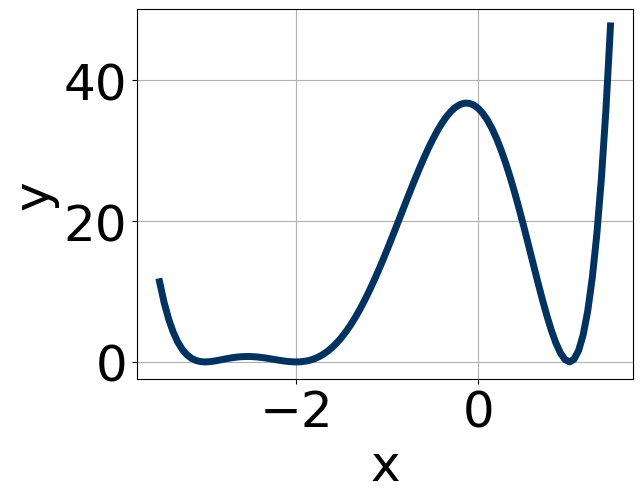
\includegraphics[width=0.5\textwidth]{../Figures/polyGraphToFunctionC.png}
\end{center}


The solution is \( 6(x + 2)^{8} (x - 1)^{6} (x + 3)^{10} \), which is option A.\begin{enumerate}[label=\Alph*.]
\item \( 6(x + 2)^{8} (x - 1)^{6} (x + 3)^{10} \)

* This is the correct option.
\item \( 2(x + 2)^{10} (x - 1)^{4} (x + 3)^{5} \)

The factor $(x + 3)$ should have an even power.
\item \( 16(x + 2)^{8} (x - 1)^{9} (x + 3)^{7} \)

The factors $(x - 1)$ and $(x + 3)$ should both have even powers.
\item \( -12(x + 2)^{6} (x - 1)^{6} (x + 3)^{6} \)

This corresponds to the leading coefficient being the opposite value than it should be.
\item \( -12(x + 2)^{10} (x - 1)^{10} (x + 3)^{11} \)

The factor $(x + 3)$ should have an even power and the leading coefficient should be the opposite sign.
\end{enumerate}

\textbf{General Comment:} General Comments: Draw the x-axis to determine which zeros are touching (and so have even multiplicity) or cross (and have odd multiplicity).
}
\litem{
Describe the zero behavior of the zero $x = -6$ of the polynomial below.
\[ f(x) = 5(x - 8)^{9}(x + 8)^{6}(x - 6)^{14}(x + 6)^{9} \]The solution is the graph below, which is option A.
\begin{center}
    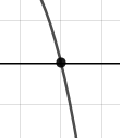
\includegraphics[width=0.3\textwidth]{../Figures/polyZeroBehaviorCopyAC.png}
\end{center}\begin{enumerate}[label=\Alph*.]
\begin{multicols}{2}
\item 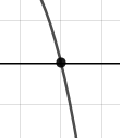
\includegraphics[width = 0.3\textwidth]{../Figures/polyZeroBehaviorCopyAC.png}
\item 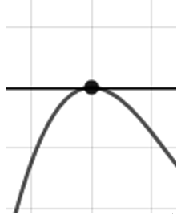
\includegraphics[width = 0.3\textwidth]{../Figures/polyZeroBehaviorCopyBC.png}
\item 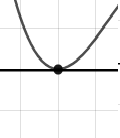
\includegraphics[width = 0.3\textwidth]{../Figures/polyZeroBehaviorCopyCC.png}
\item 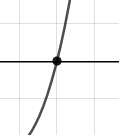
\includegraphics[width = 0.3\textwidth]{../Figures/polyZeroBehaviorCopyDC.png}
\end{multicols}\item None of the above.\end{enumerate}
\textbf{General Comment:} You will need to sketch the entire graph, then zoom in on the zero the question asks about.
}
\litem{
Describe the zero behavior of the zero $x = 2$ of the polynomial below.
\[ f(x) = 3(x - 2)^{3}(x + 2)^{8}(x + 5)^{6}(x - 5)^{7} \]The solution is the graph below, which is option A.
\begin{center}
    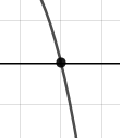
\includegraphics[width=0.3\textwidth]{../Figures/polyZeroBehaviorAC.png}
\end{center}\begin{enumerate}[label=\Alph*.]
\begin{multicols}{2}
\item 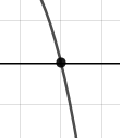
\includegraphics[width = 0.3\textwidth]{../Figures/polyZeroBehaviorAC.png}
\item 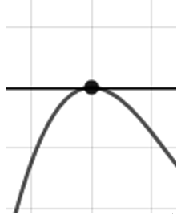
\includegraphics[width = 0.3\textwidth]{../Figures/polyZeroBehaviorBC.png}
\item 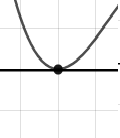
\includegraphics[width = 0.3\textwidth]{../Figures/polyZeroBehaviorCC.png}
\item 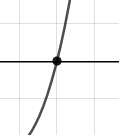
\includegraphics[width = 0.3\textwidth]{../Figures/polyZeroBehaviorDC.png}
\end{multicols}\item None of the above.\end{enumerate}
\textbf{General Comment:} You will need to sketch the entire graph, then zoom in on the zero the question asks about.
}
\litem{
Construct the lowest-degree polynomial given the zeros below. Then, choose the intervals that contain the coefficients of the polynomial in the form $x^3+bx^2+cx+d$.
\[ 5 + 3 i \text{ and } 1 \]The solution is \( x^{3} -11 x^{2} +44 x -34 \), which is option D.\begin{enumerate}[label=\Alph*.]
\item \( b \in [7, 14], c \in [43.1, 45.1], \text{ and } d \in [32.85, 34.42] \)

$x^{3} +11 x^{2} +44 x + 34$, which corresponds to multiplying out $(x-(5 + 3 i))(x-(5 - 3 i))(x + 1)$.
\item \( b \in [-4, 2], c \in [-6.2, -5.8], \text{ and } d \in [4.36, 5.61] \)

$x^{3} + x^{2} -6 x + 5$, which corresponds to multiplying out $(x -5)(x -1)$.
\item \( b \in [-4, 2], c \in [-4.9, -1.2], \text{ and } d \in [1.56, 3.56] \)

$x^{3} + x^{2} -4 x + 3$, which corresponds to multiplying out $(x -3)(x -1)$.
\item \( b \in [-13, -2], c \in [43.1, 45.1], \text{ and } d \in [-35.09, -33.44] \)

* $x^{3} -11 x^{2} +44 x -34$, which is the correct option.
\item \( \text{None of the above.} \)

This corresponds to making an unanticipated error or not understanding how to use nonreal complex numbers to create the lowest-degree polynomial. If you chose this and are not sure what you did wrong, please contact the coordinator for help.
\end{enumerate}

\textbf{General Comment:} Remember that the conjugate of $a+bi$ is $a-bi$. Since these zeros always come in pairs, we need to multiply out $(x-(5 + 3 i))(x-(5 - 3 i))(x-(1))$.
}
\litem{
Construct the lowest-degree polynomial given the zeros below. Then, choose the intervals that contain the coefficients of the polynomial in the form $ax^3+bx^2+cx+d$.
\[ \frac{2}{3}, \frac{-3}{2}, \text{ and } \frac{-5}{3} \]The solution is \( 18x^{3} +45 x^{2} +7 x -30 \), which is option A.\begin{enumerate}[label=\Alph*.]
\item \( a \in [18, 20], b \in [44, 49], c \in [4, 9], \text{ and } d \in [-33, -23] \)

* $18x^{3} +45 x^{2} +7 x -30$, which is the correct option.
\item \( a \in [18, 20], b \in [10, 22], c \in [-45, -37], \text{ and } d \in [-33, -23] \)

$18x^{3} +15 x^{2} -43 x -30$, which corresponds to multiplying out $(3x + 2)(2x -3)(3x + 5)$.
\item \( a \in [18, 20], b \in [44, 49], c \in [4, 9], \text{ and } d \in [22, 35] \)

$18x^{3} +45 x^{2} +7 x + 30$, which corresponds to multiplying everything correctly except the constant term.
\item \( a \in [18, 20], b \in [-52, -44], c \in [4, 9], \text{ and } d \in [22, 35] \)

$18x^{3} -45 x^{2} +7 x + 30$, which corresponds to multiplying out $(3x + 2)(2x -3)(3x -5)$.
\item \( a \in [18, 20], b \in [69, 80], c \in [79, 85], \text{ and } d \in [22, 35] \)

$18x^{3} +69 x^{2} +83 x + 30$, which corresponds to multiplying out $(3x + 2)(2x + 3)(3x + 5)$.
\end{enumerate}

\textbf{General Comment:} To construct the lowest-degree polynomial, you want to multiply out $(3x -2)(2x + 3)(3x + 5)$
}
\litem{
Describe the end behavior of the polynomial below.
\[ f(x) = 7(x - 2)^{4}(x + 2)^{7}(x + 7)^{4}(x - 7)^{4} \]The solution is the graph below, which is option D.
\begin{center}
    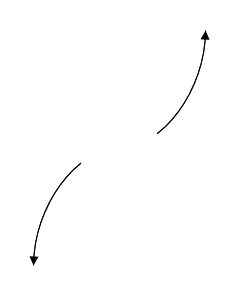
\includegraphics[width=0.3\textwidth]{../Figures/polyEndBehaviorCopyDC.png}
\end{center}\begin{enumerate}[label=\Alph*.]
\begin{multicols}{2}
\item 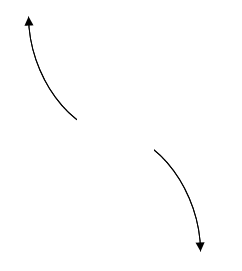
\includegraphics[width = 0.3\textwidth]{../Figures/polyEndBehaviorCopyAC.png}
\item 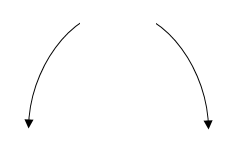
\includegraphics[width = 0.3\textwidth]{../Figures/polyEndBehaviorCopyBC.png}
\item 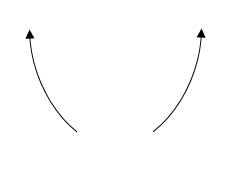
\includegraphics[width = 0.3\textwidth]{../Figures/polyEndBehaviorCopyCC.png}
\item 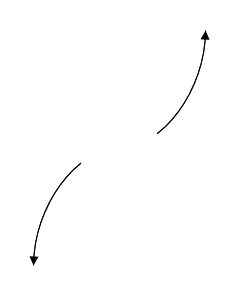
\includegraphics[width = 0.3\textwidth]{../Figures/polyEndBehaviorCopyDC.png}
\end{multicols}\item None of the above.\end{enumerate}
\textbf{General Comment:} Remember that end behavior is determined by the leading coefficient AND whether the \textbf{sum} of the multiplicities is positive or negative.
}
\litem{
Which of the following equations \textit{could} be of the graph presented below?

\begin{center}
    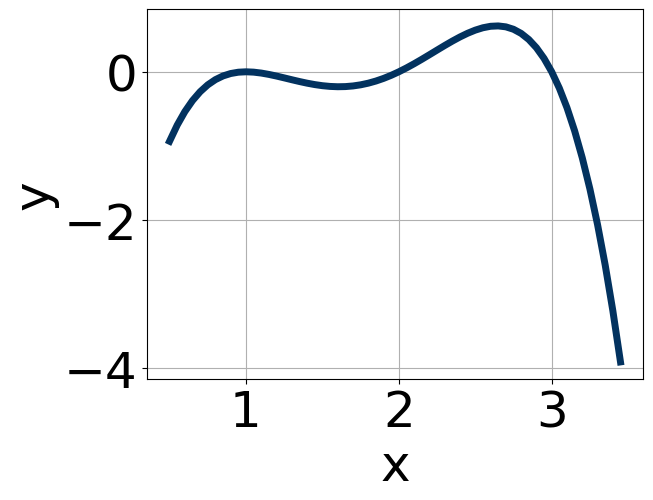
\includegraphics[width=0.5\textwidth]{../Figures/polyGraphToFunctionCopyC.png}
\end{center}


The solution is \( -2(x - 1)^{4} (x - 2)^{5} (x - 3)^{11} \), which is option B.\begin{enumerate}[label=\Alph*.]
\item \( 10(x - 1)^{6} (x - 2)^{11} (x - 3)^{5} \)

This corresponds to the leading coefficient being the opposite value than it should be.
\item \( -2(x - 1)^{4} (x - 2)^{5} (x - 3)^{11} \)

* This is the correct option.
\item \( -10(x - 1)^{8} (x - 2)^{6} (x - 3)^{9} \)

The factor $(x - 2)$ should have an odd power.
\item \( -18(x - 1)^{7} (x - 2)^{10} (x - 3)^{7} \)

The factor $1$ should have an even power and the factor $2$ should have an odd power.
\item \( 19(x - 1)^{10} (x - 2)^{7} (x - 3)^{8} \)

The factor $(x - 3)$ should have an odd power and the leading coefficient should be the opposite sign.
\end{enumerate}

\textbf{General Comment:} General Comments: Draw the x-axis to determine which zeros are touching (and so have even multiplicity) or cross (and have odd multiplicity).
}
\litem{
Describe the end behavior of the polynomial below.
\[ f(x) = 6(x - 3)^{5}(x + 3)^{8}(x + 6)^{2}(x - 6)^{2} \]The solution is the graph below, which is option D.
\begin{center}
    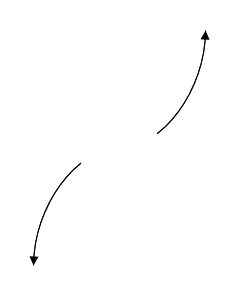
\includegraphics[width=0.3\textwidth]{../Figures/polyEndBehaviorDC.png}
\end{center}\begin{enumerate}[label=\Alph*.]
\begin{multicols}{2}
\item 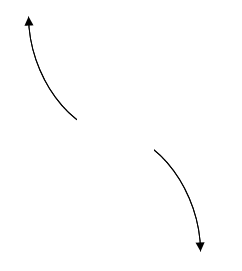
\includegraphics[width = 0.3\textwidth]{../Figures/polyEndBehaviorAC.png}
\item 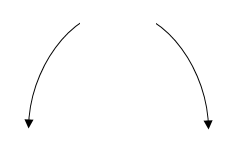
\includegraphics[width = 0.3\textwidth]{../Figures/polyEndBehaviorBC.png}
\item 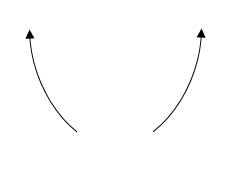
\includegraphics[width = 0.3\textwidth]{../Figures/polyEndBehaviorCC.png}
\item 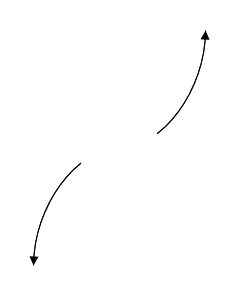
\includegraphics[width = 0.3\textwidth]{../Figures/polyEndBehaviorDC.png}
\end{multicols}\item None of the above.\end{enumerate}
\textbf{General Comment:} Remember that end behavior is determined by the leading coefficient AND whether the \textbf{sum} of the multiplicities is positive or negative.
}
\end{enumerate}

\end{document}